\section{Possible Performance Gains from Model Fragmentation}

In this section, we analyse the performance gains from optimal model fragmentation. Even though these gains will never be achievable for real applications (in most cases), the results in this section provide a theoretical lower bound. The results also help to benchmark (existing) fragmentation strategies. 

In this section, we will only analyse the time efficiency for partially loading a fragmented model. Partially loading a model is needed for the modelling traversing, querying, and loading parts of a model.

First, we need to define a few basic operations and performance functions for these operations. The operations needed to load a fragmented model are accessing a model fragment and parsing the fragment (this includes reading the persistent version of the fragment). 

We define the $parse$ function that determines how long it takes to parse a serialized model fragment of a given $size$ as a linear function: $parse(size)=\mathcal{O}\left(size\right)$. The next function $access$ determines how long it takes to find an entry in a key-value data store based on the number of key $\#keys$, i.e. number of entries: $access(\#keys)=\mathcal{O}log(\#keys)$.
Note that all data stores (key-value, files-systems, relational data bases) perform logarithmically at best \markus{cite?}.

To replace the $\mathcal{O}$-notation with actual function parameters, we measured the performance of EMF parsing (depending on model size) and HBase data store access (depending on number of data store entries). The results are shown in Fig.~\ref{fig:optimal_load_times_measured}. As expected the parsing performance is linear and the data store access behaves logarithmic. 

We can estimate the execution times for loading a part of a fragmented model for different fragment sizes. We will use the following parameters: The total model $size$, the average number of objects per fragment $fsize$, and the size of the model part that is loaded $lsize$. We assume \emph{optimal fragmentation}. In an optimal fragmentation (with respect to loading a model part), the number of objects that are actually loaded is minimal. We only need to load as many fragments as are needed to accumulate the size of the loaded model part. The time $t$ to load from an optimally fragmented model is:

$$t=\frac{lsize}{fsize}\left(access(\frac{size}{fsize}) + parse(fsize)\right)$$

With functions $parse$ and $access$ as determined by our measurements, we get the times presented in Fig.~\ref{fig:optimal_load_times_measured}.The contour plot shows the relation between fragment size, load size, and the time it takes to load. The contours show loads that take the same time. The linear or logarithmic parts of the contours are more or less dominant: if parsing is relatively slow, fragmentation becomes more important (linear parts of contours are longer), if accessing the data-base becomes relatively slow, fragmentation becomes less relevant and generally large fragment sizes are more desirable (logarithmic parts of contours are longer).

From this plot, we can see what fragmentation allows compared to no fragmentation ($fsize=size$) or complete fragmentation ($fsize=1$). No fragmentation always takes the full time. Of course optimal results can be obtained if ($lsize=fsize$). This optimal result allows to load models a 1000 times bigger at the same time than total fragmentation. 

\begin{figure}[ht]
\begin{minipage}[b]{0.5\linewidth}
\centering
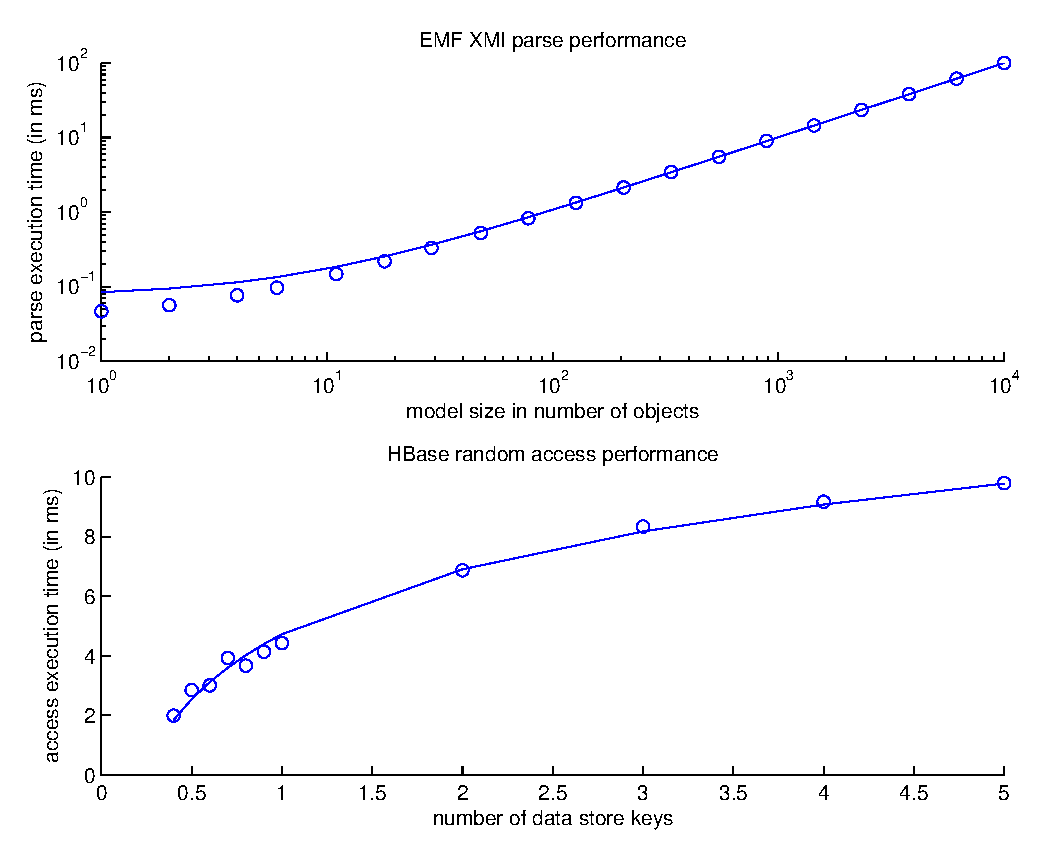
\includegraphics[width=\linewidth]{figures/emfHbasePerf}
\caption{Measure for liner parsing performance of EMF and logarithmic access performance of HBase.}
\label{fig:figures/emf_hbase_performance_measured}
\end{minipage}
\hspace{0.5cm}
\begin{minipage}[b]{0.5\linewidth}
\centering
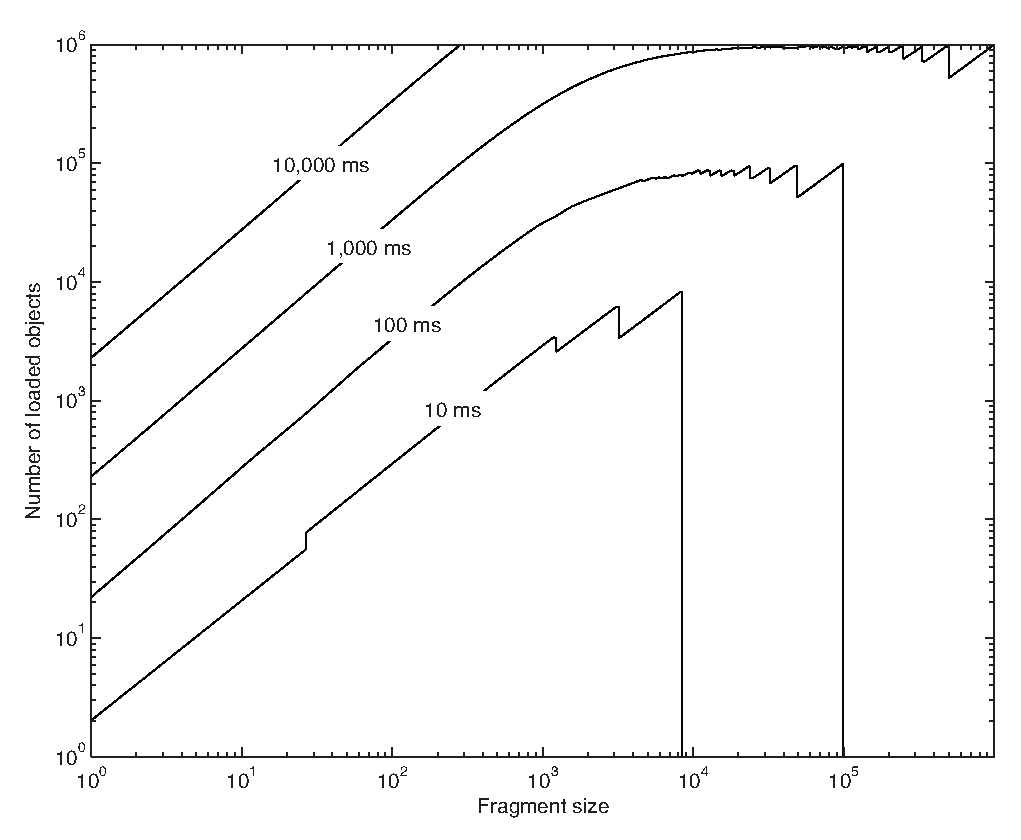
\includegraphics[width=\linewidth]{figures/fragTheoryContour}
\caption{Load times based on actual EMF parsing and HBase access measurements.}
\label{fig:optimal_load_times_measured}
\end{minipage}
\end{figure}

\begin{figure}
\centering
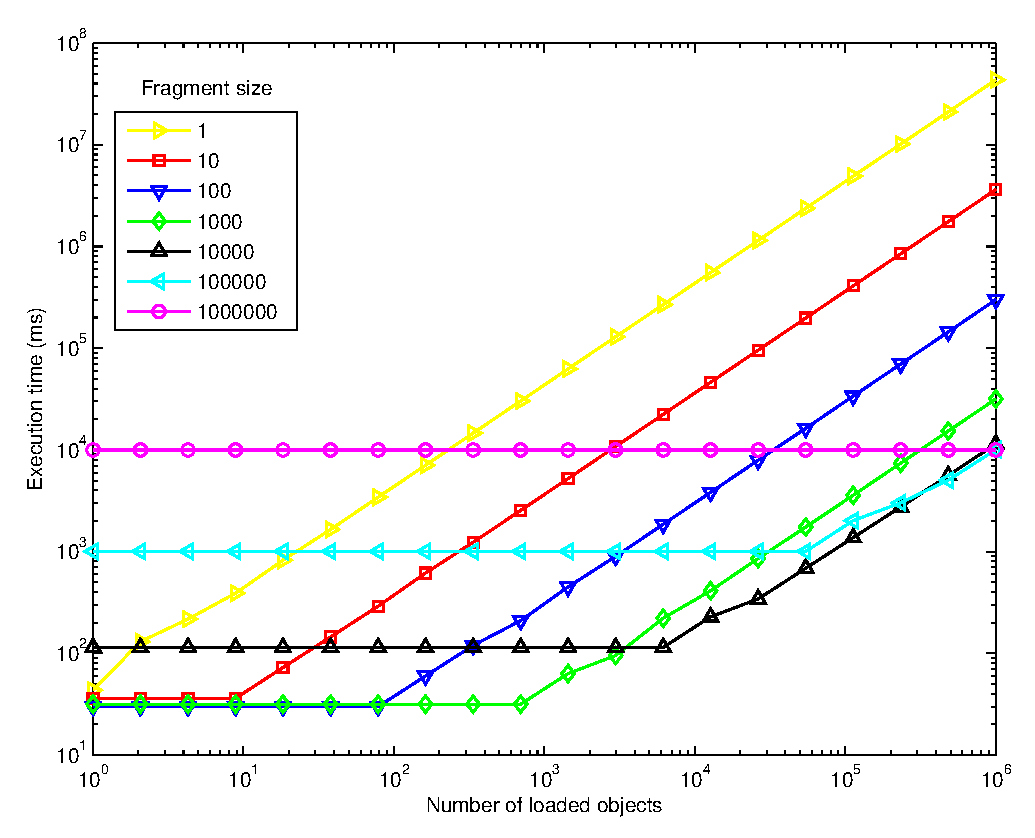
\includegraphics[width=0.65\linewidth]{figures/fragTheory}
\caption{Load times based on actual EMF parsing and ...}
\end{figure}

In this analysis, we only considered unsorted, non distributed key-value stores. Sorted key-value stores further allow to organise fragments in the order that they are most often loaded in. This reduces the number of necessary logarithmic accesses and replaces them with time constant accesses (scans). Distributed key-value stores allow to access and read fragments in parallel, thus allowing shorter execution times. \markus{Refer to future work?}